\setcounter{chapter}{5}
\chapter{Dynamique}
\section{Les Forces}
\subsection{Généralités}

\blocrouge{Définition}{Une force est une action mécanique modélisée par un vecteur $\vec{F}$. Une force est décrite avec la donnée de 4 caractéristiques:

\begin{enumerate}
	\item Point d'application 
	\item Direction
	\item Sens
	\item Valeur
\end{enumerate}}
\subsection{Exemples}
\subsection*{Le poids}

\blocrouge{Définition}{
Le poids $\vec{P}$ d'un système de masse m est la force d'attraction exercée par la Terre sur le système.\\
Caractéristiques :
\begin{itemize}
\item Direction : \trou{verticale}
\item Sens : \trou{vers le bas}
\item Point d'application : \trou{le centre d'inertie du système}
\item Valeur : \trou{$P=m \times g$} avec \\
P \trou{la force en Newton (N)}, m  \trou{la masse en kilogramme (kg)}, et g  \trou{l'intensité de la pesanteur en $\si{\newton\per\kilo\gram}$}
\end{itemize}
}

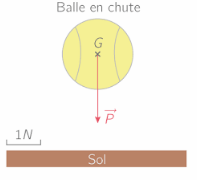
\includegraphics[scale=0.6]{figures/dynamique/poids2}


\subsection*{La réaction d'un support}
\begin{minipage}{0,3\linewidth}
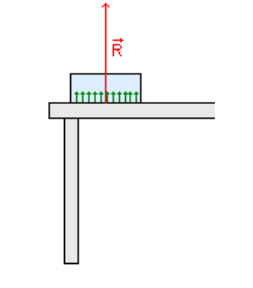
\includegraphics[scale=0.5]{figures/dynamique/reaction}
\end{minipage}
\begin{minipage}{0,7\linewidth}
La force exercée par un support sur un système en contact ($\vec{F}_{support/systeme}$) est encore appelée la \trou{réaction $\vec{R}$} du système.\\
\\
Pour un système immobile ou en mouvement sans frottement sur une surface lisse, les caractéristiques de cette force notée $\vec{R_N}$ pour réaction normale sont : 
\begin{itemize}
\item Point d'application : \trou{centre de la surface en contact}
\item direction :  \trou{perpendiculaire au support}
\item Sens : \trou{orientée du support vers le système.}
\item valeur : \trou{à déterminer selon les cas, notée R.}
\end{itemize}
\end{minipage}


\begin{minipage}{0,3\linewidth}
\includegraphics[scale=0.9]{figures/dynamique/fig1b}
\end{minipage}
\begin{minipage}{0.7\linewidth}

Lorsqu'il y a des frottements, s'ajoute à cette réaction normale $\vec{R_N}$ la réaction tangentielle $\vec{R_T}$, parallèle à la surface de contact et qui modélise les frottements, donc qui s'oppose au mouvement.
\end{minipage}

\blocrouge{A retenir}{ La force $\vec{R}$ exercée par un support sur le système se décompose en général en une somme de 2 vecteurs: $$ \overrightarrow{R}=\trou{\overrightarrow{R_N}}+\trou{\overrightarrow{R_T}}$$ Si les frottements sont négligés  $\overrightarrow{R}=  \overrightarrow{R_N}$ car  $\trou{\overrightarrow{R_T}=\vec{0}}$}

\etiquette{Remarque} Parfois on note $\vec{N}$ le vecteur $\overrightarrow{R_N}$ et $\vec{T}$ le vecteur $\overrightarrow{R_T}$. Attention, rien à voir avec les vecteurs de la base de Frenet.%image réaction normale et réaction tangentielle à trouver
\subsection*{La tension d'un fil}


\begin{minipage}{0,3\linewidth}
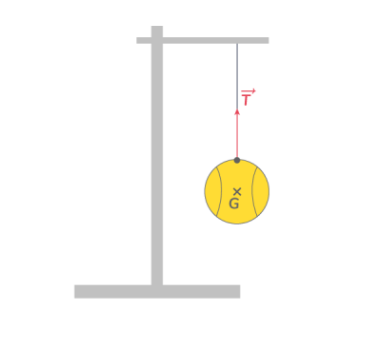
\includegraphics[scale=0.5]{figures/dynamique/tension}
\end{minipage}
\begin{minipage}{0,7\linewidth}
La force exercée par un fil sur un système en contact ($\vec{F}_{fil/systeme}$) est encore appelée la tension $\vec{T}$ d'un fil.\\
\\
Les caractéristiques de cette force sont : 
\begin{itemize}
\item Point d'application : \trou{point d'accroche du système au fil}
\item direction :  \trou{celle du fil}
\item Sens : \trou{orientée du point d'accroche vers le fil.}
\item valeur : \trou{à déterminer selon les cas, notée T.}
\end{itemize}
\end{minipage}

\section{Lois de Newton}
\subsection{Centre de masse}
Les lois de Newton qui vont suivre s'appliquent au centre de masse\footnote{centre de masse = centre d'inertie} G du système. Il s'agit du point où se situe la position\footnote{De manière rigoureuse c'est le barycentre du système. En pratique, il est généralement au centre du système.} moyenne des masses constituant le système. \\
Le centre de masse G est le point du système qui décrit la trajectoire la plus simple.

\etiquette{Ex 11 p 229}

\subsection{Première loi ou principe d'inertie}

Un système est isolé si il n'est soumis à \trou{aucune force} (vue de l'esprit).\\ Un système est pseudo isolé si les forces qu'il subit se compensent c'est à dire: $$\sum \vec{F}= \trou{\vec{F_1} + \vec{F_2}+...} =\vec{0}$$
Subir des forces qui se compensent c'est comme ne pas subir de forces.

\blocrouge{Principe d'inertie}{Dans un référentiel galiléen, si le système est isolé ou pseudo isolé alors son mouvement est \trou{rectiligne uniforme}. Et réciproquement.
\\Formulation mathématique: $$\sum \vec{F}=\trou{\vec{0} } \Leftrightarrow \vec{v} = \trou{\vec{cst}}$$
}

\paragraph*{Remarques} 
Un référentiel est galiléen si le principe d'inertie est parfaitement vérifié dans ce référentiel.\\
Le sol est un référentiel galiléen à condition que l'expérience ne dure pas trop longtemps afin de pouvoir négliger la rotation propre de la Terre\footnote{ Il faut aussi que la masse du système soit faible devant la masse des océans afin de négliger les effets de marées. }

 \etiquette{Réciproque } 
 Si le système est en MRU ou immobile alors d'après le \trou{principe d'inertie} on peut conclure que  les forces se \trou{compensent}.
 
 
 \etiquette{Application 1} Faire l'exercice 1 de la fiche

\subsection{2nde loi de Newton ou relation fondamentale de la dynamique}

\blocrouge{2nde Loi de Newton}{

Dans un référentiel galiléen, l'accélération et les forces subies par le système de masse m sont reliées par:
 $$\sum \vec{F}= \vec{F_1} + \vec{F_2}+... = m\times \vec{a(t)}$$
 
 }
 
 
 \etiquetterouge{Stratégie importante}
 
 Si on connaît les forces appliquées au système, on peut calculer le vecteur $\vec{a}(t)$. Puis, en cherchant des primitives on trouve les coordonnées des vecteurs vitesse et position.
 \vspace{1cm}

\newpage
 \etiquette{Application 2: Détermination du mouvement à partir des forces}
 
Faire l'exercice 2 de la fiche.\\

\subsection{3ème loi de Newton: Principe des actions réciproques}

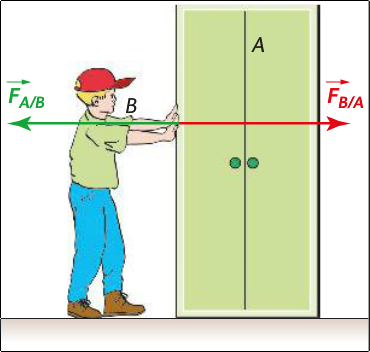
\includegraphics[scale=0.3]{figures/dynamique/fig3}\\
\blocrouge{Enoncé}{A et B sont deux objets en interaction. La force exercée par A sur B est \trou{l'opposée} de la force exercée par B sur A. Ces deux forces ont la même \trou{valeur}, la même \trou{direction}, mais sont de sens \trou{opposés}}
\vspace{1cm}

\etiquette{Capacités Exigibles}
\begin{itemize}
	\item Justifier qualitativement la position du centre de masse d’un système, cette position étant donnée.
	\item Discuter qualitativement du caractère galiléen d’un référentiel donné pour le mouvement étudié.
	\item Utiliser la deuxième loi de Newton dans des situations variées pour en déduire :\\
- le vecteur accélération du centre de masse, les forces appliquées au système étant connues ;\\
- la somme des forces appliquées au système, le mouvement du centre de masse étant connu.
\end{itemize}
 
 \etiquette{Exercices à faire} Voir fiche d'exercices

\includepdf[pages=-]{figures/dynamique/exos_lois_de_newton.pdf}
 
  